\section{Backend}\label{sec:poc:backend}
\begin{figure}[ht]
  \centering
  %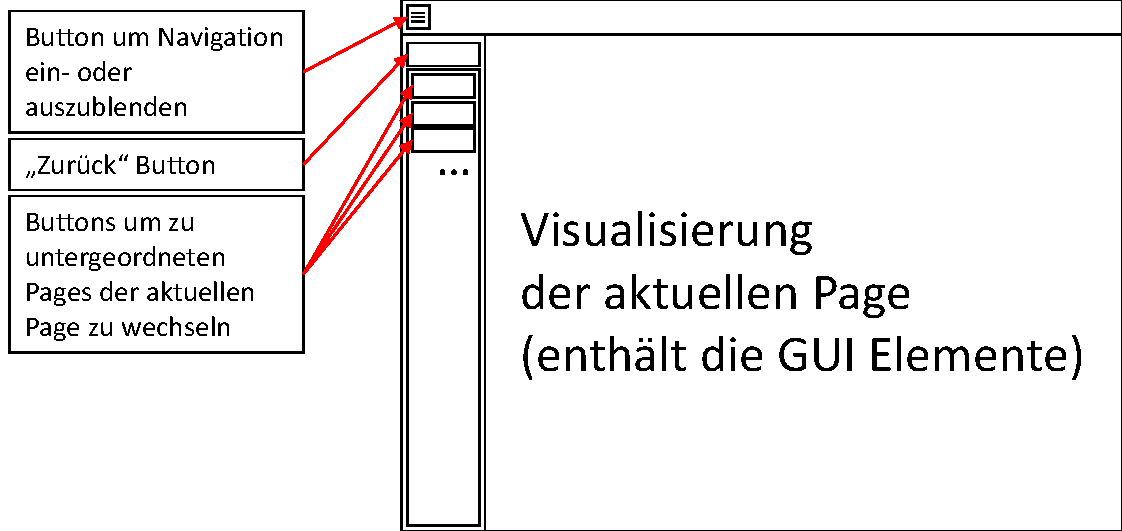
\includegraphics[width=\textwidth]{content/hauptteil/systemEntwurf/res/LayoutFrontend.pdf} DA DES MINIMALIFIZIERTE DIAG REIN
  \caption[Klassediagramm Backend]{Klassediagramm}
  \label{fig:backend:classDiag}
\end{figure}
%beschreibung diagramm
%erwähnung datenaustausch zwischen basisklassen zu abgeleitetrer...(dispatcher.... )
  %endlich anzahl an fkt für daten backend -> basisklassen
  %pro basisklasse ein dispatcher im Backend (virtual) --> Verweis auf Kapitel
%erwähnung message klassen die geparsed wwerden


\subsection{WebsocketServer}
%kurze Erwähnung sinn der klasse
%datenaustausch zwischen WebsocketServer zu abgeleitetrer...(dispatcher.... ) (I/O)
%beschreibung msg klasse mit diagram
%dispatcher codeausschnitt
%beschreibung dispatcher
\subsection{SqlClient}
%kurze Erwähnung sinn der klasse
%datenaustausch zwischen SqlClient zu abgeleitetrer...(dispatcher.... ) (I/O)
%beschreibung msg klasse mit diagram
%dispatcher codeausschnitt
%beschreibung dispatcher
\subsection{OpcuaServer}
%kurze Erwähnung sinn der klasse
%datenaustausch zwischen OpcuaServer zu abgeleitetrer...(dispatcher.... ) (I/O)
%beschreibung msg klasse mit diagram
%dispatcher codeausschnitt
%beschreibung dispatcher